% vim:ft=tex
% rubber: module xelatex

\subsection{Face feature extraction}
\label{sec:features}

We build on the SURF extractor discussed in section~\ref{sec:features-prior}. An open-source implementation of this algorithm is OpenSURF, described in \cite{OpenSURF}. OpenCV also includes its own implementation of the SURF algorithm. We integrated both these versions into our application, and have also added our own implementation of SURF. Our implementation is inspired by (and is therefore structured similarly to) the OpenSURF implementation.

\subsubsection{Implementation notes}
Our implementation uses the response layers and filter sizes from \cite{SURF}. This limits the range of possible values for the `octaves' and `intervals' parameters to (1-5) and (3-4) respectively. The OpenSURF implementation simply ignores the `intervals' parameter in its calculations. The process of estimating the determinant of the Hessian matrix from the filter response values requires a weight for the $D_{xy}$ direction. We follow \cite{SURF} in setting this weight to $0.9$.

Note that the three implementations (ours, OpenCV and OpenSURF) use different threshold values for the algorithm. It appears\footnote{ with the caveat that it is difficult to tell because the OpenCV code is rather convoluted.} that OpenCV does not area-normalise the threshold values. This is very likely the reason for the discrepancy between our implementation and that of OpenCV. OpenSURF represents greyscale values as floating point values between 0 and 1, whereas we represent them as int values between 0 and 255. This would appear to account for the discrepancy between our threshold values and those of OpenSURF.

The interpolation between points to get subpixel accuracy for interest points follows the method in \cite{inv-features}. This method essentially amounts to solving a linear system using pixel differences as approximations for the derivatives. In \cite{SURF}, it is implied that this process should be used to iteratively interpolate keypoint locations, and discard those that do not converge. However, both OpenCV and OpenSURF appear to simply use the interpolation deltas to discard keypoints that interpolate to a different point, rather than attempting to iterate towards convergence. Our program follows these implementations in abandoning the iterative paradigm. We found, though, that using interpolation for subpixel accuracy \emph{at all} appears to make our implementation `worse', in as far as it causes the output of our algorithm to diverge from that of the OpenCV and OpenSURF implementations. Why this should be the case is unclear.

\subsubsection{Experimental process}

\paragraph{Experimental parameters.}
To test the capability of our own SURF algorithm implementation, we ran it on six images of human faces. Credit is given to the Massachusetts Institute of Technology and to the Center for Biological and Computational Learning for providing the database of facial images; see \cite{database}. The forward-facing images subset of the MIT-CBCL database was used. We first manually extracted features from the original images, identifying 10 interest points (eye centres, eye corners, mouth corners, mouth centre, tip of nose) in each case.

\begin{figure} [h]
  \centering
  \subfloat[Face image 1]{ \label{fig:face-1} 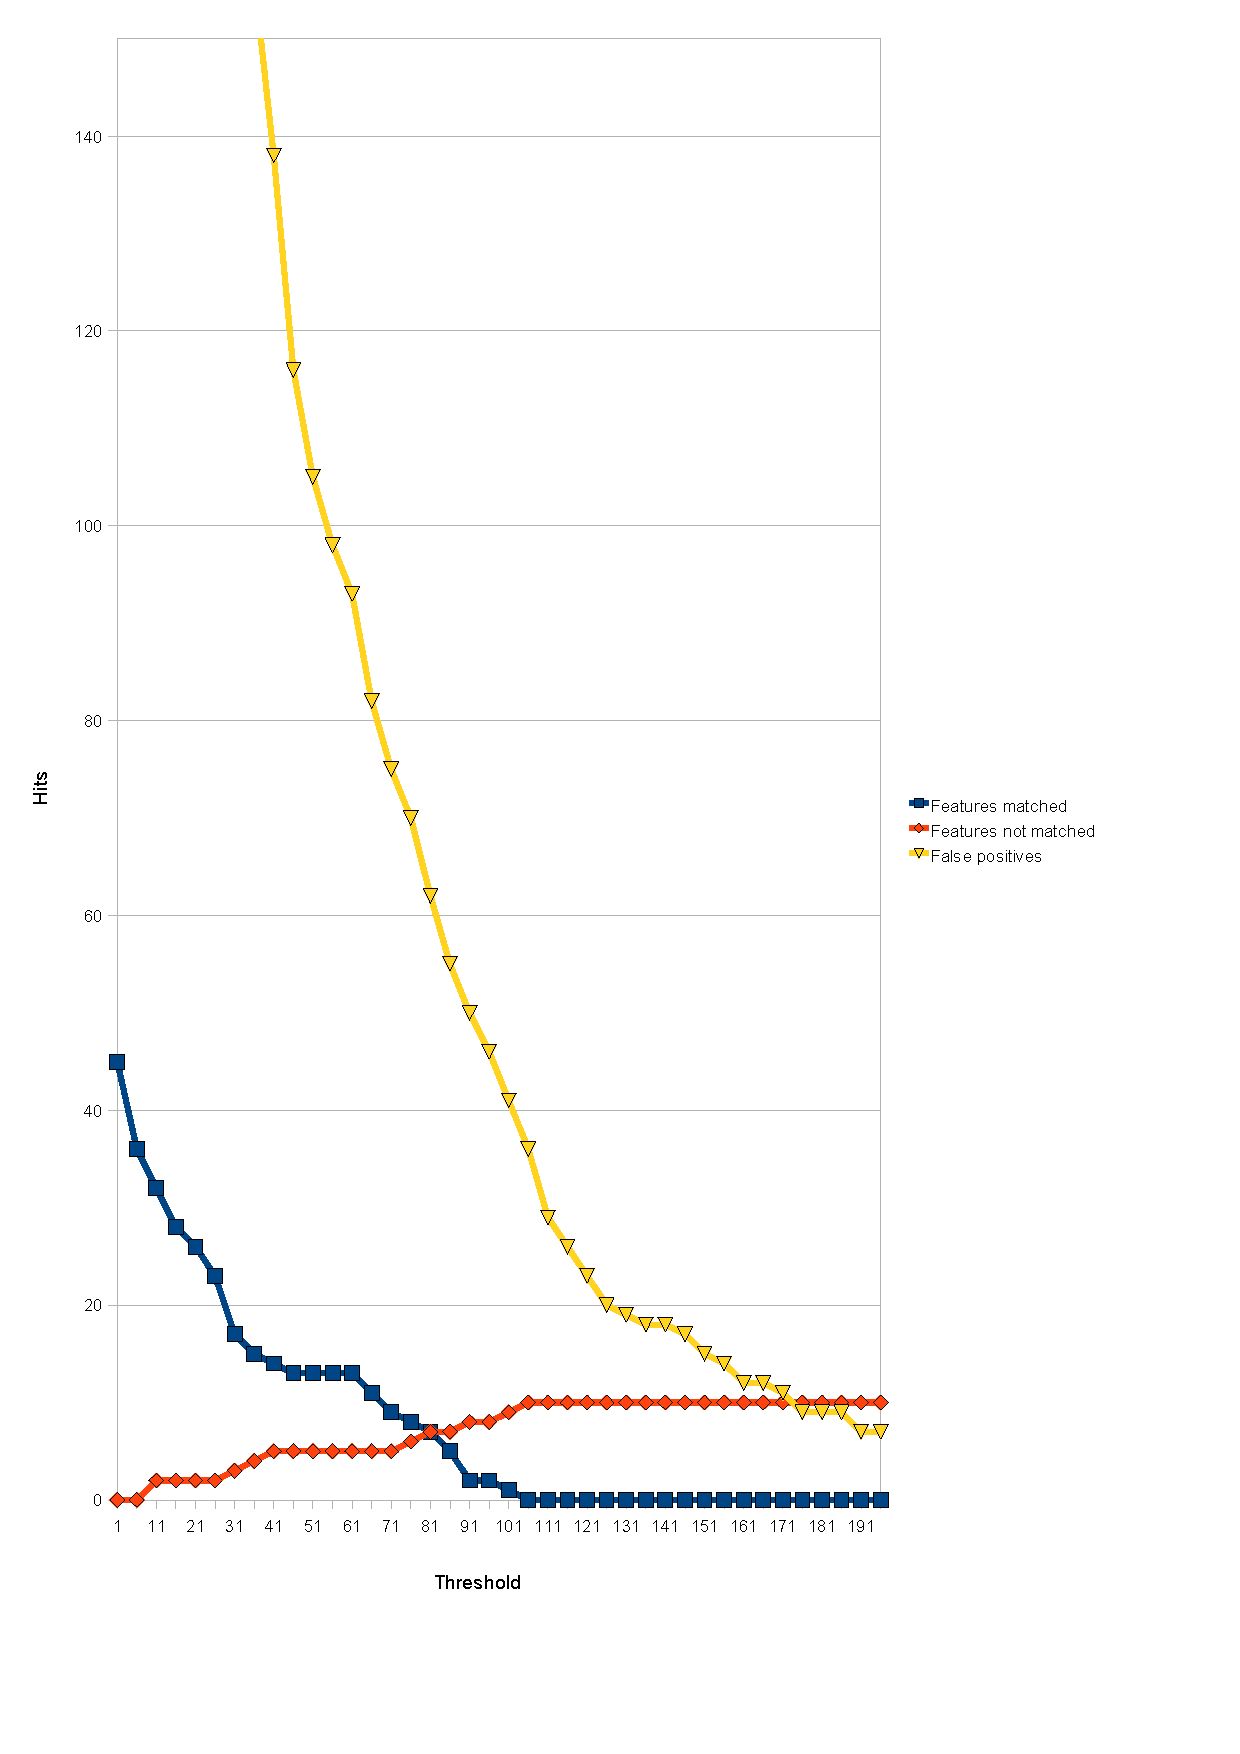
\includegraphics[height=0.27\textheight, width=0.9\textwidth]{figures/face1} }\\
  \subfloat[Face image 2]{ \label{fig:face-2} 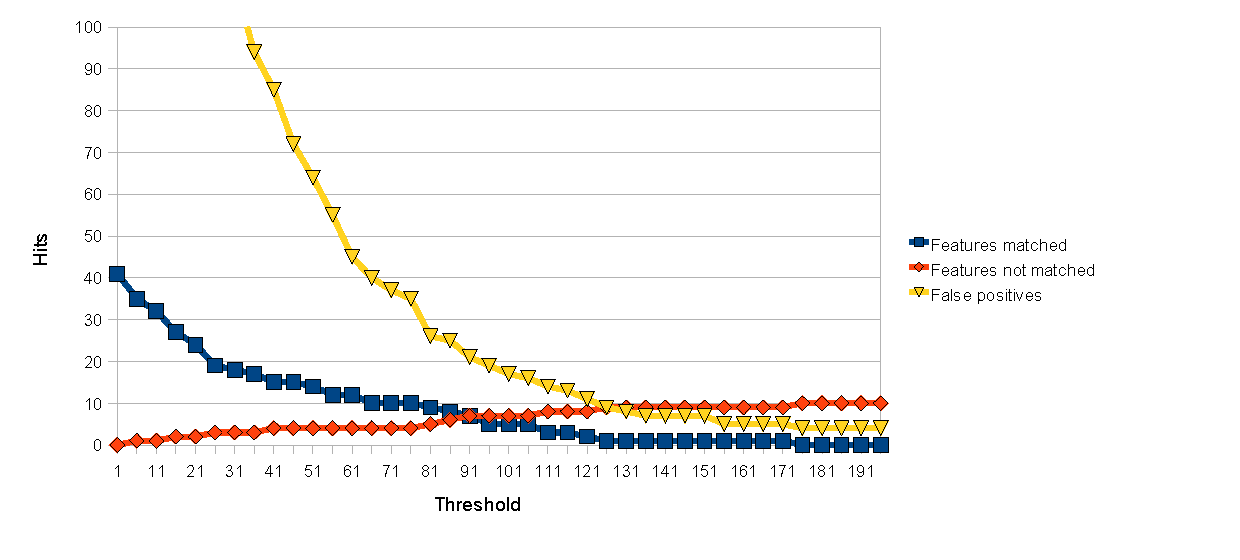
\includegraphics[height=0.27\textheight, width=0.9\textwidth]{figures/face2} }
  \caption[Face features identified by our SURF implementation (images 1 \& 2)]{Face features identified by our implementation of the SURF algorithm. Each chart shows the true positives, false negatives and false positives for one test image.}
  \label{fig:face-features-hits-1}
\end{figure}

For each face, we tested 40 threshold values (from 1 to 196, increasing by a gradation of 5 each time). We noted the number of interest points returned that correctly identify features; for this purpose we count an interest point that ``hits" within 15 pixels of the manually identified feature as a success). As well as these true positives, we also investigated the number of false negatives (faces features which the algorithm fails to return interest points for) and false positives (other points which the algorithm incorrectly identifies as features\footnote{ i.e. returned interest points which do not lie within 15 pixels of a manually identified feature point.}).

\begin{figure} [h]
  \centering
  \subfloat[Face image 3]{ \label{fig:face-3} 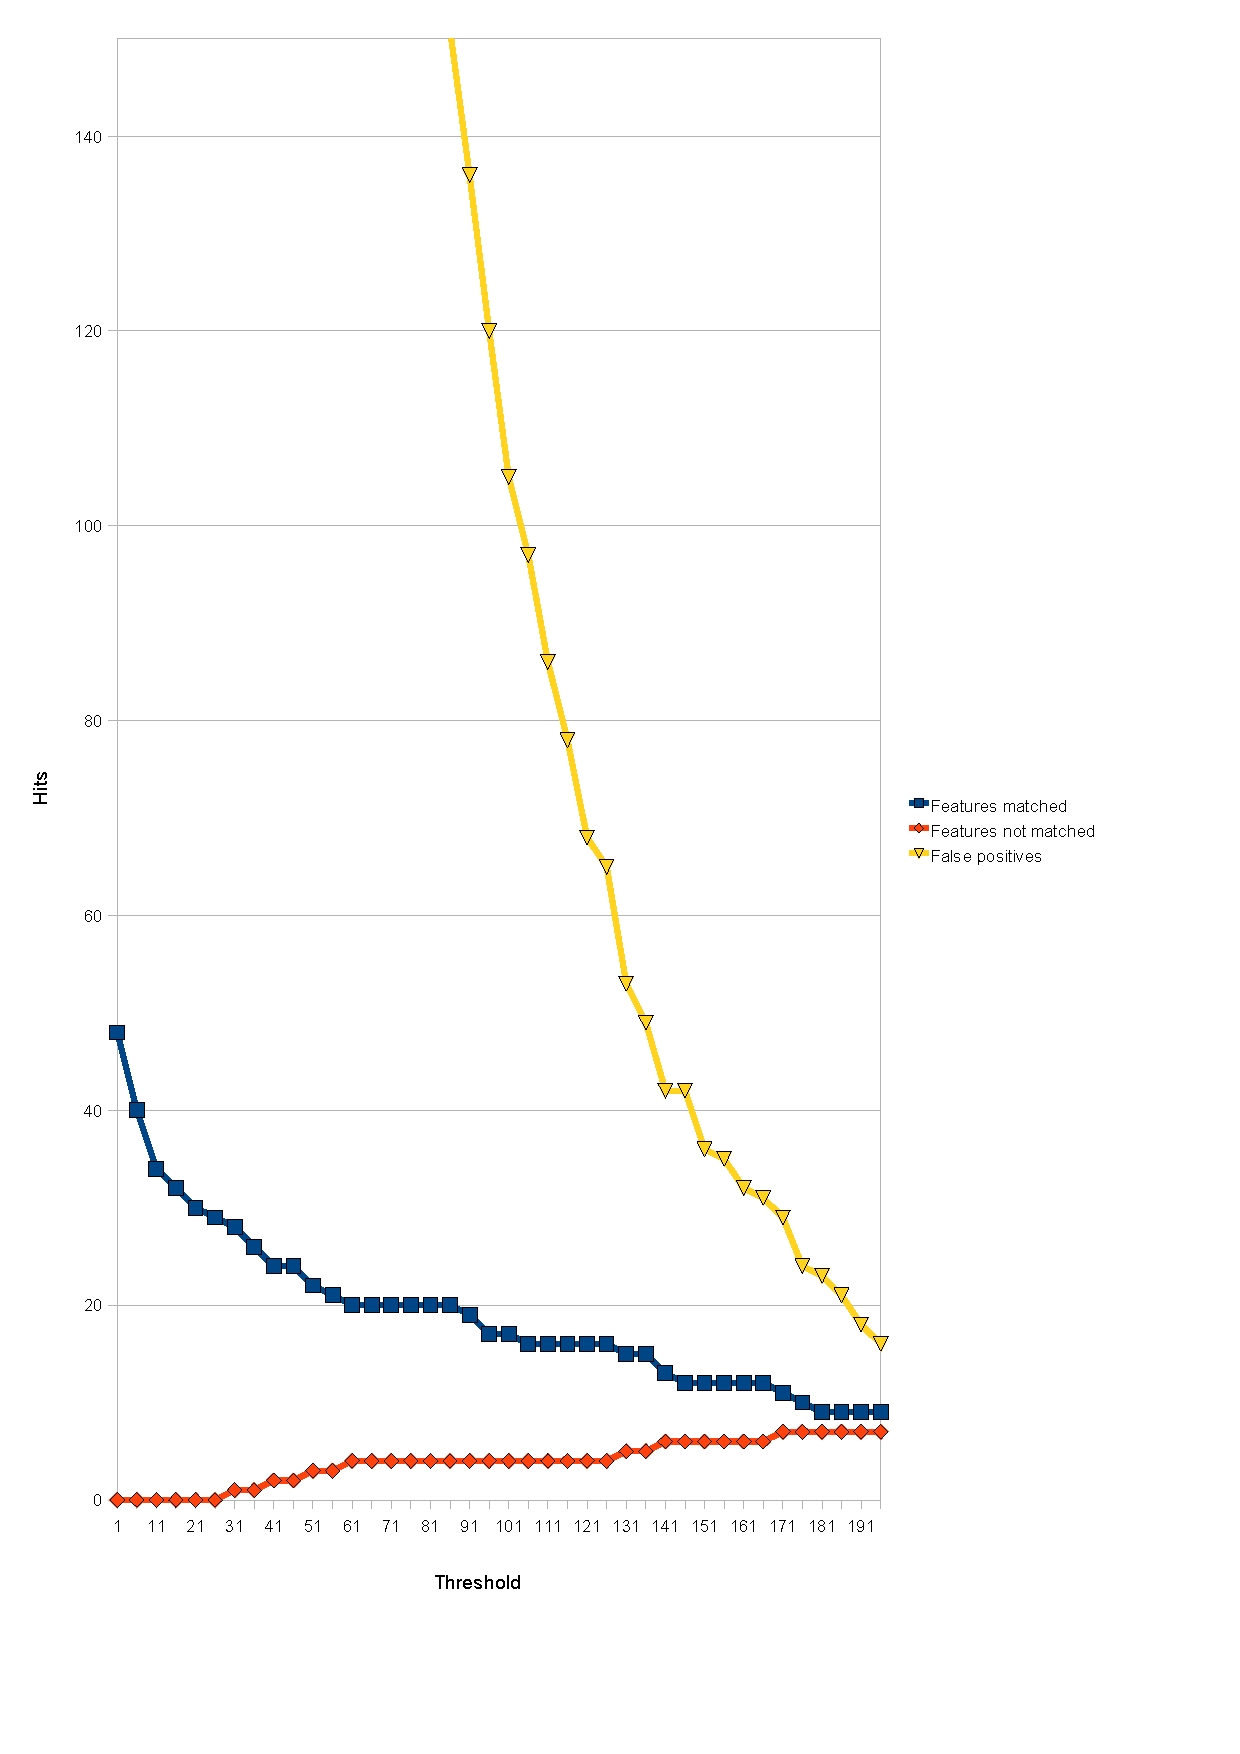
\includegraphics[height=0.27\textheight, width=0.9\textwidth]{figures/face3} }\\
  \subfloat[Face image 4]{ \label{fig:face-4} 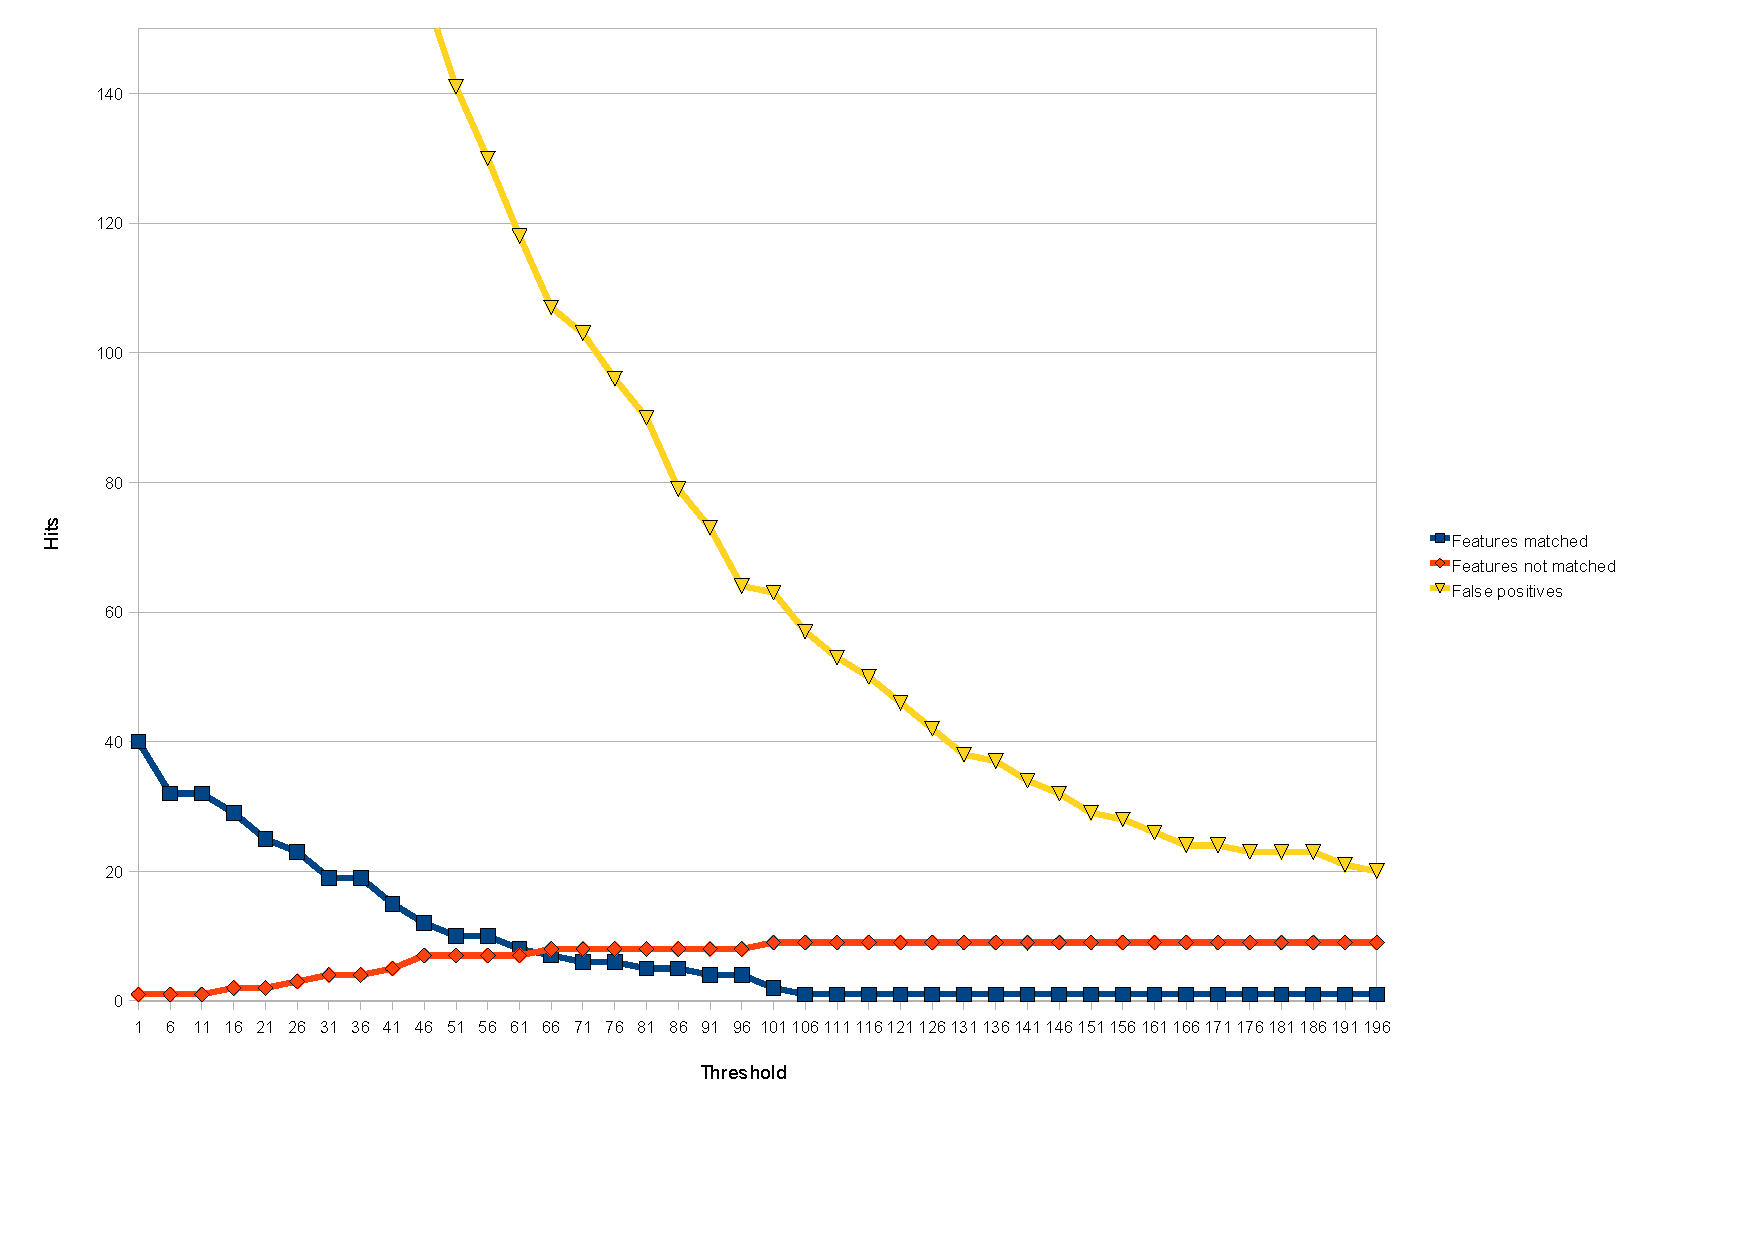
\includegraphics[height=0.27\textheight, width=0.9\textwidth]{figures/face4} }
  \caption[Face features identified by our SURF implementation (images 3 \& 4)]{Face features identified by our implementation of the SURF algorithm. Each chart shows the true positives, false negatives and false positives for one test image.}
  \label{fig:face-features-hits-2}
\end{figure}

\paragraph{Experimental results.}
We present the results of our testing in figures~\ref{fig:face-features-hits-1}, ~\ref{fig:face-features-hits-2} and ~\ref{fig:face-features-hits-3}. The charts therein plot the changes in feature extraction success, false negatives, and false positives. Note that we manually defined only $10$ features per face image. This is considerably smaller than the number of ``interesting" features on a human face; for this reason, false positives tend to dominate the interest points returned. In fact, the magnitude of the false positives could not always be represented on the graphs without increasing the scale so much that the other values would become indistinguishable from zero; we have therefore placed an artificial limit of 150 on the Y axes.

\begin{figure} [h]
  \centering
  \subfloat[Face image 5]{ \label{fig:face-5} 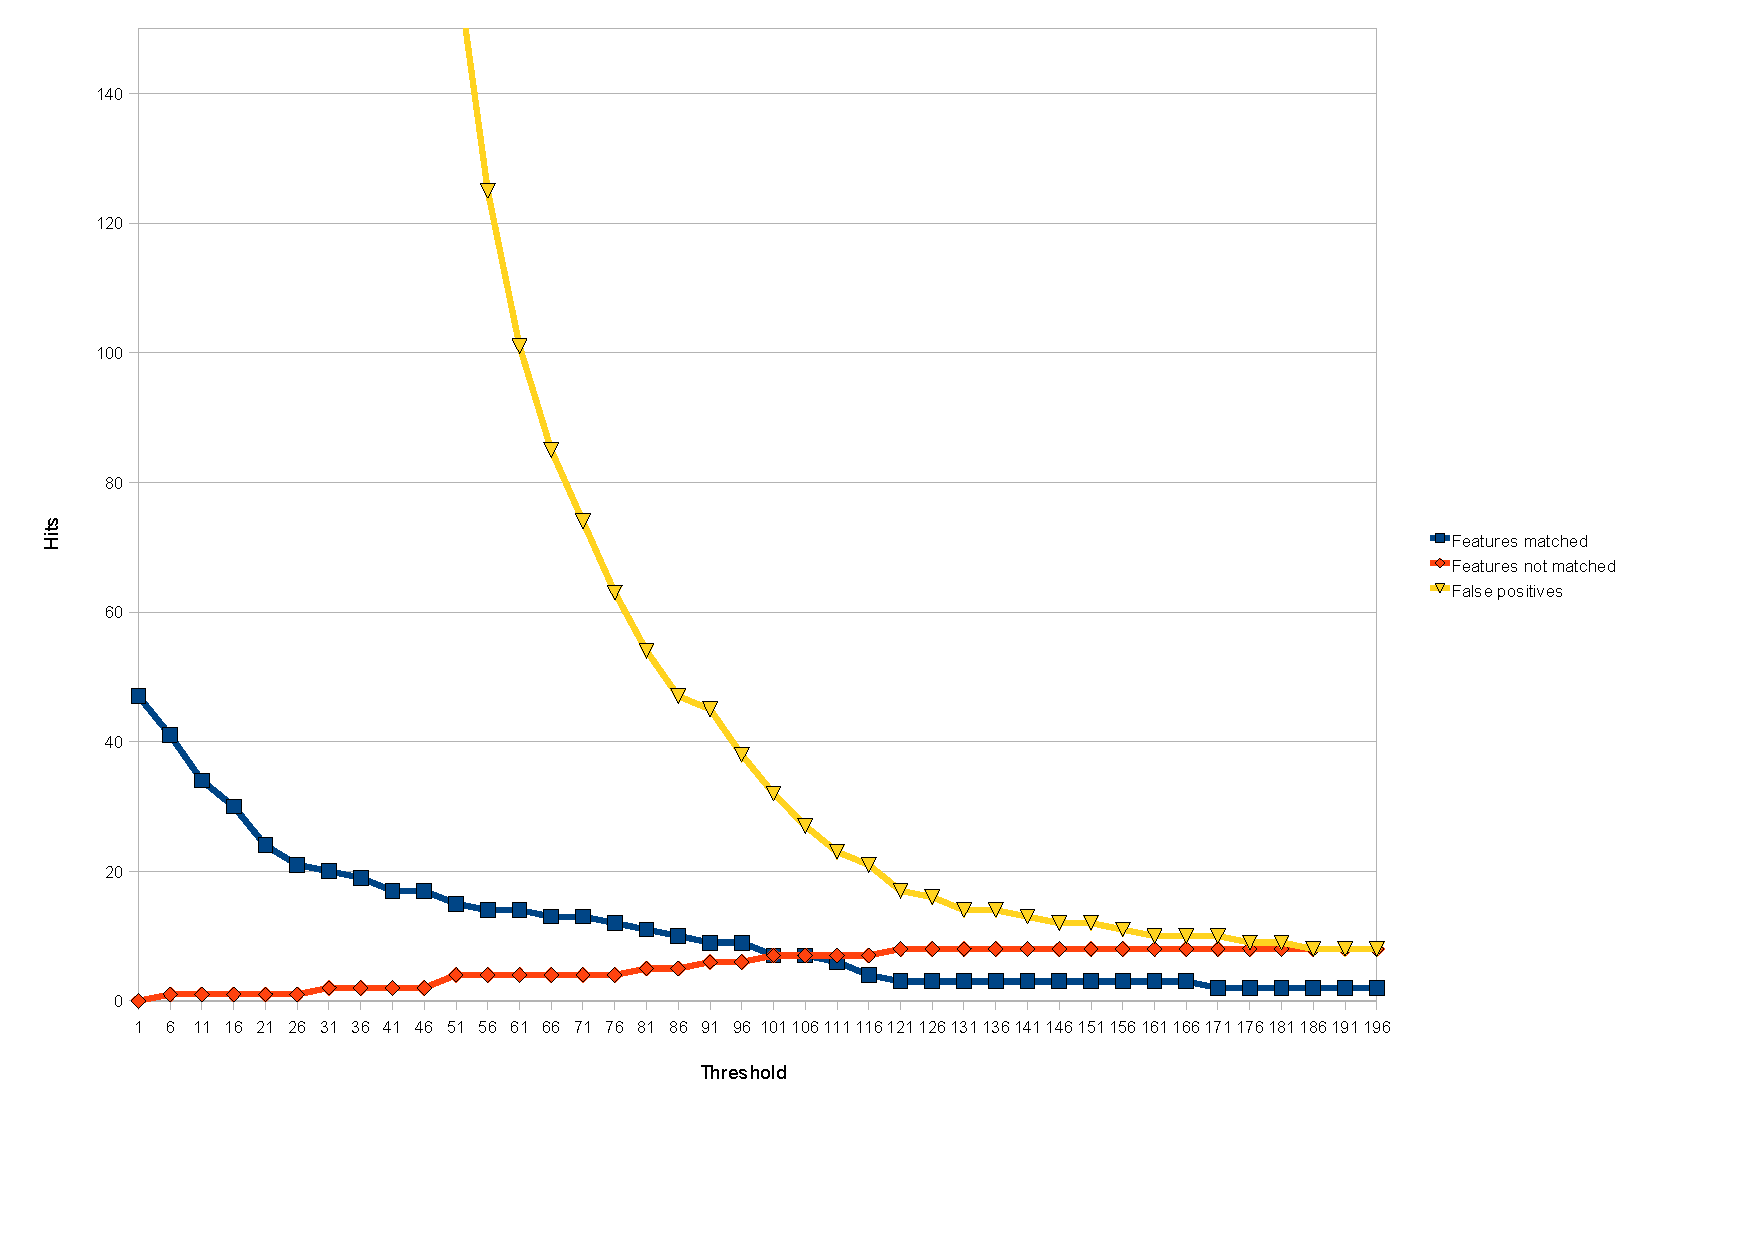
\includegraphics[height=0.27\textheight, width=0.9\textwidth]{figures/face5} }\\
  \subfloat[Face image 6]{ \label{fig:face-6} 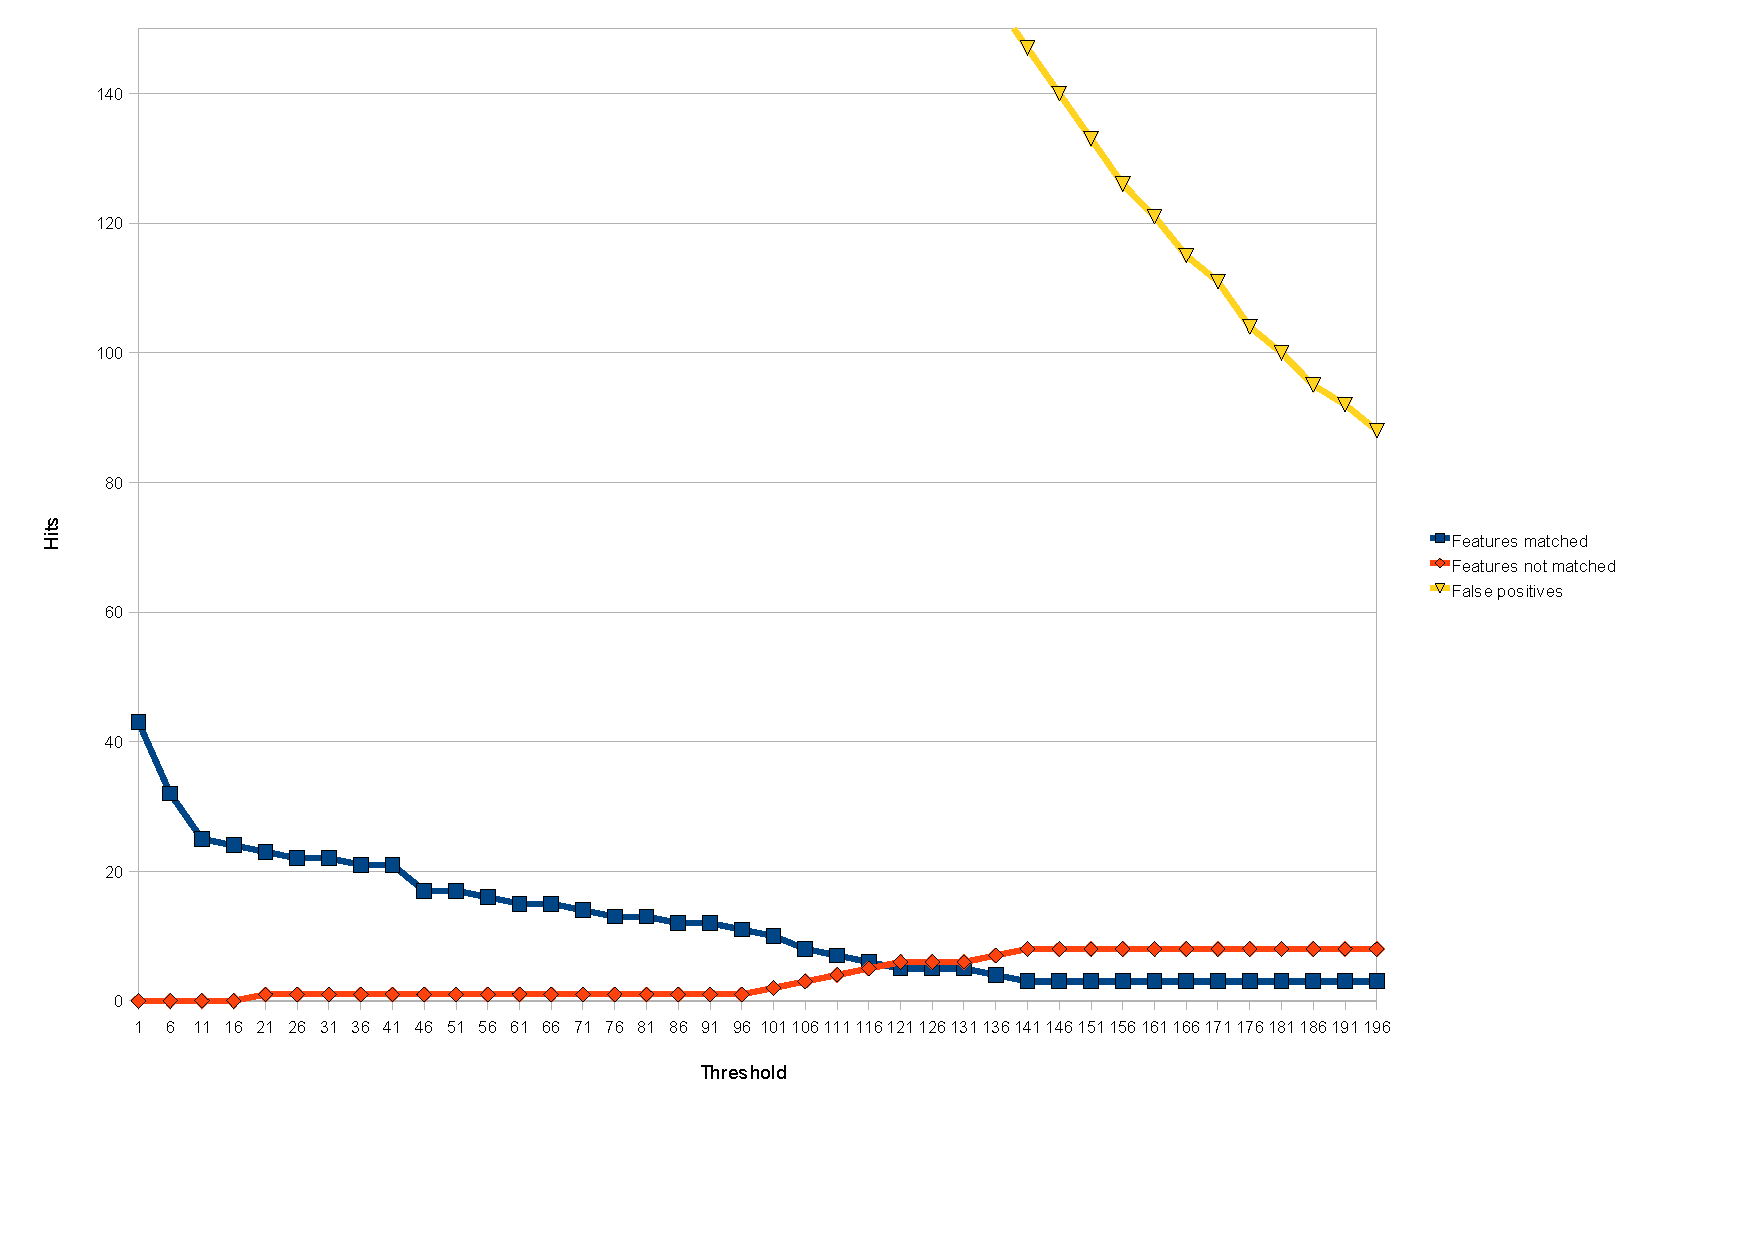
\includegraphics[height=0.27\textheight, width=0.9\textwidth]{figures/face6} }
  \caption[Face features identified by our SURF implementation (images 5 \& 6)]{Face features identified by our implementation of the SURF algorithm. Each chart shows the true positives, false negatives and false positives for one test image.}
  \label{fig:face-features-hits-3}
\end{figure}

\paragraph{Conclusions.}
As expected, when the threshold increases, the total number of interest points returned decreases. There are fewer false positives, but there are also fewer genuine matches. For most of the images, half of the manually identified features are not being found by the time the threshold reaches 50. There is considerable variability between the results for the six faces. For instance, face image \#6 (figure~\ref{fig:face-6}) acquires a vast number of false positives. The performance of the algorithm on face image \#1 (figure~\ref{fig:face-1}) drops to a zero success rate much earlier than the others. Face image \#3 (figure~\ref{fig:face-3}) is unique in that it continues to match many interest points to 1 or 2 face features even at the maximum tested threshold. There is also a 
general variability of the threshold point at which the algorithm returns more false negatives (features missed) than true positives (interest points identified correctly corresponding to features). This is as low as 66 in (figure~\ref{fig:face-4}) and is higher than the tested range in (figure~\ref{fig:face-3}). This variability is expected, given the extreme heterogeneity of the human face.
